% Chapter 1

\chapter{Bulk SnSe} % Main chapter title

\label{Chapter5} % For referencing the chapter elsewhere, use \ref{Chapter1} 

%----------------------------------------------------------------------------------------

% Define some commands to keep the formatting separated from the content 
%\newcommand{\keyword}[1]{\textbf{#1}}
%\newcommand{\tabhead}[1]{\textbf{#1}}
%\newcommand{\code}[1]{\texttt{#1}}
%\newcommand{\file}[1]{\texttt{\bfseries#1}}
%\newcommand{\option}[1]{\texttt{\itshape#1}}

%----------------------------------------------------------------------------------------

\section{Introduction}

Thermoelectricity is a technologically interesting material property that allows to transform residual heat into useful electricity\cite{goldsmid2010introduction,behnia2015fundamentals}. The efficiency of this energy 
transformation is controlled by the dimensionless figure of merit
\begin{equation}
ZT=\frac{S^{2}\sigma T}{\kappa},
\end{equation}
where $S$ is the Seebeck coefficient, $\sigma$ the electrical conductivity, $T$ the temperature, and $\kappa=\kappa_{e}+\kappa_{l}$ the sum of electronic $\kappa_{e}$ and lattice $\kappa_{l}$ thermal conductivities. Therefore, a 
good thermoelectric performance requires a high power factor $P_{F}=S^{2}\sigma$ together with a low thermal conductivity. \\

Monochalcogenides have proven to be efficient thermoelectric materials\cite{heremans2008enhancement,zhang2013high,yang2008nanostructures,cho2011thermoelectric} mainly due to their strongly anharmonic lattice that implies a low 
lattice thermal conductivity\cite{delaire2011giant,li2014phonon,iizumi1975phase,o2017inelastic,ribeiro2018strong}. PbTe is an appropiate example of potential technological relevance of thermoelectric monochalcogenides: it shows 
a high $ZT$ in the $600-800$ K temperature range\cite{ravich2013semiconducting}, as high as $2.2$ when nanostructured\cite{hsu2004cubic}, and has been successfully applied in spacecrafts\cite{rowe2018thermoelectrics}. In the last 
years SnSe has attracted a great deal of attention since it was measured to be the most efficient intrinsic thermoelectric material\cite{zhao2014ultralow}. Its figure of merit soars to $2.6$ after a structural phase 
transition\cite{zhao2014ultralow,adouby1998structure,chattopadhyay1986neutron,von1981high,chatterji2018soft} at around $800$ K from the low-symmetry $Pnma$ phase to the high-symmetry $Cmcm$. See Fig. \ref{pnma-cmcm} for the crystal 
structure of the two phases.
\begin{figure}[h]
\begin{center}
\includegraphics[width=0.8\linewidth]{Figures/pnma-cmcm.pdf}
\caption{SnSe crystal structure in the a) $Pnma$ and b) $Cmcm$ phases.}
\label{pnma-cmcm}
\end{center}
\end{figure}
In the high-symmetry phase the band gap is reduced without affecting the ultralow thermal conductivity, providing the record $ZT$. \\

The phase transition takes the system from the orthorhombic $Pnma$ phase to a more symmetric base-centered orthorhombic $Cmcm$ structure. The order of the phase transition is not clear: some works\cite{zhao2014ultralow,
adouby1998structure,chattopadhyay1986neutron,chatterji2018soft} claim it is a second-order phase transition and others\cite{von1981high} it has a first-order character. A recent work\cite{dewandre2016two} argues that the transition occurs in 
two steps, where increasing temperature induces first a change in the lattice parameters that induces after a lattice instability. There is an inelastic scattering experiment for the high-temperature phase, which shows a prominent phonon collapse at the transition temperature, which suggests that the transition is of the second-order type\cite{chatterji2018soft}. \\

The most interesting thermoelectric properties appear in the high-temperature phase, where the reduction of the electronic band gap increases the number of carriers providing a higher $P_{F}$, while the thermal conductivity 
remains very low. The value of the intrinsic $\kappa_{l}$ of SnSe remains controversial, as the extremely low isotropic $0.3$ W/mK values at $800$ K reported by Zhao et al.\cite{zhao2014ultralow} could not be reproduced in 
other experiments, where a clear anisotropy is shown and the in-plane thermal conductivity is considerably larger\cite{ibrahim2017reinvestigation,sassi2014assessment,chen2014thermoelectric}. The lattice thermal conductivity 
of the $Pnma$ phase has been calculated\cite{carrete2014low,skelton2016anharmonicity} from first principles solving the BTE using harmonic phonons and 3BFC obtained perturbatively as derivatives of the BOES. The $Cmcm$ phase 
has imaginary phonons in the harmonic approximation\cite{dewandre2016two,skelton2016anharmonicity,yu2016enhanced}, as expected for the high-symmetry phase in a second-order phase transition, hindering the 
calculation of $\kappa_{l}$. \\

In this chapter we study the vibrational and thermal properties of $Cmcm$ SnSe by including anharmonicity at a non-pertubative level by using the SSCHA. We show that the phonon mode that drives the instability collapses at the 
transition temperature $T_{c}$ demonstrating that the transition is second-order. Anharmonic effects are so large that the spectral function for some in-plane modes deviates from the Lorentzian-like shape and show broad peaks, 
shoulders and satellilte peaks, as in other monochalcogenides\cite{ribeiro2018strong,li2014phonon}. We calculate the lattice thermal conductivity of $Cmcm$ SnSe by combining the anharmonic phonon spectra with perturbative and 
nonperturbative 3BFC. We show that nonperturbative anharmonic effects are not only crucial in the phonon spectra, but also in high-order force-constants, which have a huge impact on the calculated thermal conductivity. 
$\kappa_{l}$ agrees with experiments\cite{ibrahim2017reinvestigation} only with nonperturbative 3BFC.

\section{Structure and high symmetry points}

The $Cmcm$ and $Pnma$ phases are orthorhombic and their structure  is shown in Fig. \ref{pnma-cmcm}. The $Cmcm$ phase 
has a centering in the $XZ$ plane of the rectangular conventional cell and contains 4 atoms in the primitive cell. 
The primitive cell of the $Pnma$ phase contains $8$ atoms. The primitive lattice vectors 
of the $Cmcm$ structure are: $\mathbf{a}_{1}=(a/2,0,c/2)$, $\mathbf{a}_{2}=(-a/2,0,c/2)$ and
$\mathbf{a}_{3}=(0,b,0)$, where $a$ (long axis), $b$ and $c$ are the lattice constants of the conventional cell. \\

The reciprocal lattice of the $Cmcm$ phase is shown in Fig. \ref{1bzsnse}.
\begin{figure}[h]
\begin{center}
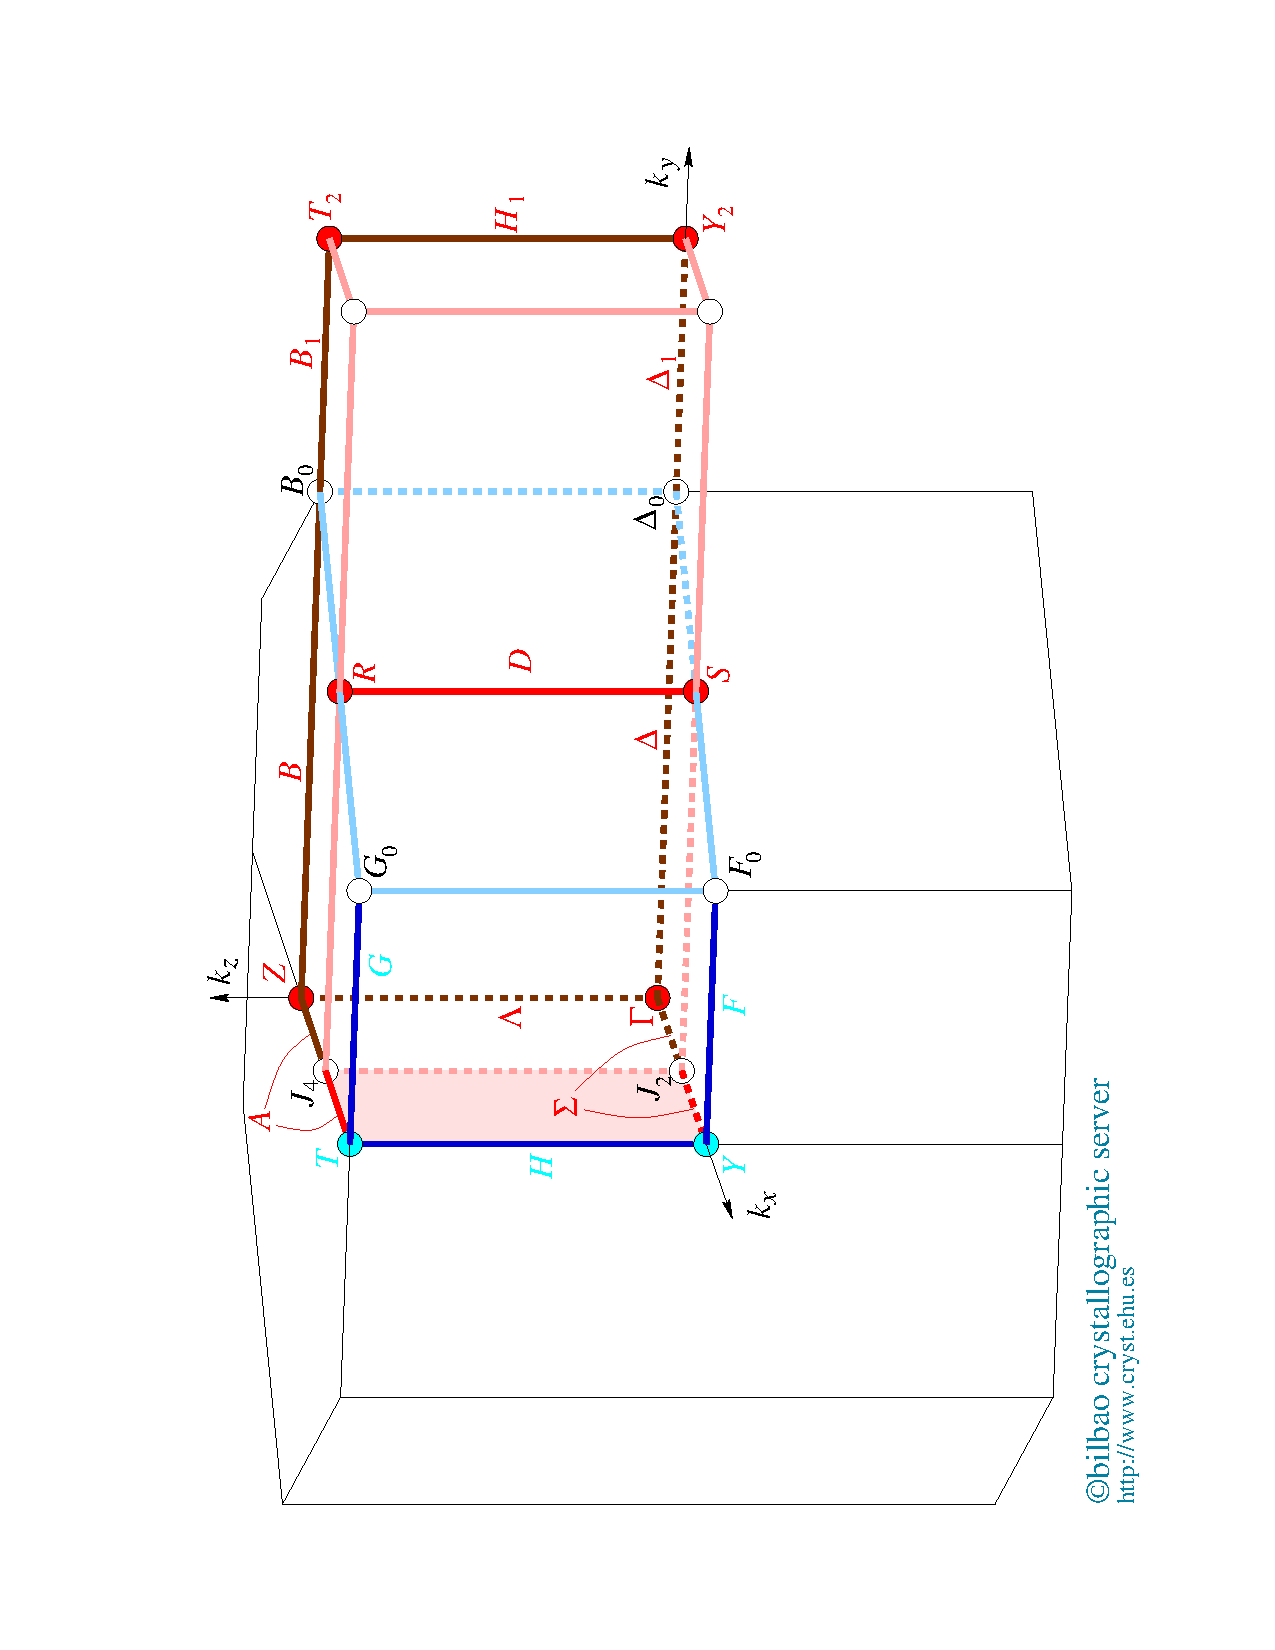
\includegraphics[width=\linewidth]{Figures/brillouinsnse.pdf}
\caption{1BZ of $Cmcm$ SnSe. The figure is taken from the Bilbao crystallographic server.}
\label{1bzsnse}
\end{center}
\end{figure}
The reciprocal lattice vectors of the $Cmcm$ primitive 1BZ are $\mathbf{b}_{1}=2\pi(1/a,0,1/c)$, 
$\mathbf{b}_{2}=2\pi(-1/a,0,1/c)$ and $\mathbf{b}_{3}=2\pi(0,1/b,0)$. The high symmetry points and their coordinates 
used in phonon dispersion figures are listed in table \ref{qpoints}.
\begin{table}
\begin{center}
\begin{tabular*}{0.45\textwidth}{l c}
 \hline
 \hline
 %\multicolumn{4}{|c|}{Country List} \\
             Symmetry point  & Reduced $\mathbf{q}$ vector  \\
 \hline
 $Z$                  &  0.0, 0.0, 0.5  \\
 $R$                  &  0.0, 0.5, 0.5  \\
 $S$                  &  0.0, 0.5, 0.0  \\
 $\Gamma$             &  0.0, 0.0, 0.0  \\
 $Y$                  &  0.5, -0.5, 0.0  \\
 $T$                  &  0.5, 0.5, 0.5  \\
 \hline
 \hline
\end{tabular*}
\end{center}
\caption[Reduced $\mathbf{q}$ vectors of the high symmetry points in the Brillouin zone of the $Cmcm$ phase.]{Reduced 
$\mathbf{q}$ vectors of the high symmetry points in the Brillouin zone of the $Cmcm$ phase. The coordinates are given 
with respect to the reciprocal lattice vectors of the primitive cell.}
\label{qpoints}
\end{table}
\\

In both phases, $Cmcm$ and $Pnma$, the Sn and Se atoms are located in the 4c Wyckoff positions. In the $Cmcm$ phase 
this Wyckoff position has only one free parameter and it is of the form ($x$,1/4,0). In the $Pnma$ phase there are 
two free parameters ($x$,1/4,$z$). When the system transforms from the $Pnma$ to the $Cmcm$ phase, the free $z$ 
parameter of the 4c Wyckoff position is forced to be in the high symmetry position. As the $Cmcm$ phase has a 
centering, this high symmetry position can be 0 or 0.5.

\section{Calculation details}

Our calculations are based on DFT using the QUANTUM-ESPRESSO\cite{giannozzi2009quantum} software package. Harmonic phonons were calculated within DFPT and perturbative 3BFC were calculated within DFPT or finite 
differences\cite{li2014shengbte}. Anharmonic phonons and nonperturbative 3BFC were calculated using the SSCHA. For the exchange-correlation interaction we use the Perdew-Burke-Ernzerhof (PBE) generalized gradient 
approximation and the local density approximation (LDA) with ultrasoft (US) and Projector Augmented Wave method (PAW) pseudopotentials respectively. Due to limitations in the implementation of perturbative 3BFC 
within DFPT we use norm-conserving (NC) pseudopotentials only for the perturbative 3BFC calculation. We use a cutoff 
energy of 70 Ry and a grid of $16\times16\times16$ $\boldsymbol{k}$ points to sample the first Brillouin zone. For 
the harmonic phonon calculations we use a $6\times6\times6$ supercell and a $2\times2\times2$ one for the 3BFC. 
We impose the acoustic sum rule to the third-order force-constants with an iterative method prior to their Fourier
interpolation\cite{paulatto2013anharmonic,aseginolaza2019phonon}. For the SSCHA calculation we use a 
$2\times2\times2$ supercell. Then, for the anharmonic phonon dispersion, we 
interpolate the difference between the harmonic and anharmonic force-constants in the $2\times2\times2$ supercell to 
the $6\times6\times6$ and we add it to the $6\times6\times6$ harmonic force-constants (see appendix \ref{appendixB} 
for more details). For the line width calculations we use a $20\times20\times20$ $\boldsymbol{q}$ points grid 
obtained by Fourier interpolation with a smearing of $1$ cm$^{-1}$. For the thermal conductivity calculation we use 
a $10\times10\times10$ grid of $\boldsymbol{q}$ points to sample the first Brillouin zone. We have done calculations 
in denser grids to test these parameters. We have done SSCHA calculations using different lattice volumes. When we talk about the "theory" (theoretical) lattice we are referring to the relaxed lattice at DFT level. When we talk about the "exp" (experimental) lattice we refer to the experimental lattice parameters at the transition temperature between the $Cmcm$ and $Pnma$ phases. The "stretched" lattice refers to a stretched lattice with respect to the "theory" in the PBE case. The lattice parameters and the experimental references are listed in table \ref{cell-parameters}. We have 
only included the effective charges in the calculation of the harmonic phonons in Figs. \ref{harmonic-volume} and 
\ref{exchangebc}. We have seen that the effect of the effective charges is negligible in the thermal conductivity. 
In order to account for the effective charges within the SSCHA, we include the effective charges in the dynamical 
matrices after the SSCHA minimization.

\section{Phase transition}

The group/subgroup index of the $Cmcm$/$Pnma$ transition is $2$, making a displacive second-order transition possible\cite{toledano1987landau}. In this scenario, the transition temperature $T_{c}$ is defined as the temperature 
at which the second derivative of the free energy $F$ with respect to the order parameter $Q$ that transforms the structure continuously from the $Cmcm$ phase $(Q=0)$ into the $Pnma$ $(Q\ne0)$ vanishes. As it was already 
pointed out\cite{chattopadhyay1986neutron}, symmetry\cite{orobengoa2009amplimodes,perez2010mode} dictates that the amplitude of the transition is dominated by the distortion pattern associated to a non-degenerate mode $(Y_{1})$
at the zone border $Y$ point with irreducible representation $Y_{2}^{+}$ (see Fig. \ref{patterns} for the distortion pattern).
\begin{figure}[h]
\begin{center}
\includegraphics[width=0.8\linewidth]{Figures/normal-modes.pdf}
\caption[Phonon eigenvector patterns.]{a) Atomic displacements of mode $\Gamma_{1}$. b) Atomic displacements of mode $Y_{2}$. c) Atomic displacements of mode $Y_{1}$.}
\label{patterns}
\end{center}
\end{figure}
This means that $\partial^{2}F/\partial Q^{2}$ is proportional to the eigenvalue of the free energy Hessian matrix associated to this irreducible representation: $\Omega^{(F)2}_{Y_{1}}$. This frequency can be calculated within the 
SSCHA using Eq. \ref{free-energy-hessian}. \\

The calculated temperature dependence of $\Omega^{(F)2}_{Y_{1}}$ is shown in Fig. \ref{freq-y1-snse} for LDA and PBE for two different lattice volumes in each case.
\begin{figure}[h]
\begin{center}
\includegraphics[width=0.9\linewidth]{Figures/freq-main-snse.eps}
	\caption[Phonon collapse in SnSe.]{$\Omega^{(F)2}_{Y_{1}}$ as a function of temperature within LDA and PBE approximations for different lattice volumes (circles). In the LDA we compare the results obtained with the theoretical and 
experimental\cite{zhao2014ultralow} lattice parameters. In the PBE calculation we present the results for the experimental lattice parameters and a stretched unit cell (see Table \ref{cell-parameters} for the lattice
parameters). The solid lines correspond to a polynomial fit.}
\label{freq-y1-snse}
\end{center}
\end{figure}
\begin{table}
\begin{center}
\begin{tabular*}{0.65\textwidth}{l c c c c c c}
 \hline
 \hline
            & $a$  & $b$  & $c$  & $P_{xx}$ & $P_{yy}$ & $P_{zz}$ \\
 \hline
 LDA theory                  &  21.58  &  7.90  & 7.90  &  0.4  &  0.6  &  0.7  \\
 LDA Exp.                    &  22.13  &  8.13  & 8.13  & -1.1  & -2.0  & -2.2  \\
 PBE theory                  &  22.77  &  8.13  & 8.13  &  0.5  &  1.1  &  1.0  \\
 PBE Exp.                    &  22.13  &  8.13  & 8.13  &  1.8  &  1.3  &  1.2  \\
 PBE Stretched               &  23.48  &  8.27  & 8.27  & -0.3  & -0.7  & -0.7  \\
 \hline
 \hline
\end{tabular*}
\end{center}
\caption[Experimental and theoretical lattice parameters of $Cmcm$ SnSe]{Experimental\cite{zhao2014ultralow} and 
	theoretical (DFT at static level) LDA and PBE lattice parameters used in this work. The stretched cell used 
	in some calculations is also given. $a$, $b$, and $c$ lattice parameters are given in Bohr length units 
	($a_0$) and the three components of the stress tensor in GPa units. The pressure is calculated including 
	vibrational terms at an anharmonic level at the following temperatures for each case: $200$ K (LDA theory), 
	$600$ K (LDA Exp.), $400$ K (PBE Exp.), $400$ K (PBE theory), and $400$ K (PBE stretched).}
\label{cell-parameters}
\end{table}
In all cases $\Omega^{(F)2}_{Y_{1}}$ is positive at high temperatures, but it rapidly decreases with lowering the temperature, vanishing at $T_{c}$. This phonon collapse is consistent with a second-order phase transition between
the $Pnma$ and $Cmcm$. We check that a SSCHA calculation at $T>T_{c}$ ($T=800$ K) starting from the relaxed low-symmetry $Pnma$ phase (relaxed at DFT static level) yields the high-symmetry $Cmcm$ atomic positions for the 
$\boldsymbol{\mathcal{R}}$ centroids. The SSCHA relaxation is shown in Fig. \ref{atomic-relaxation}.
\begin{figure}[h]
\begin{center}
\includegraphics[width=0.9\linewidth]{Figures/positions.eps}
\caption{Wyckoff $z$ parameter of the 4c Wyckoff position in the $Pnma$ phase as a function of the SSCHA 
minimization step.}
\label{atomic-relaxation}
\end{center}
\end{figure}
As we can see, the $z$ free Wyckoff parameters of the 4c Wyckoff positions of the $Pnma$ phase relaxes to the 
high symmetry positions $0$ and $0.5$. The new wyckoff position is the 4c wyckoff position of the $Cmcm$ 
phase. The error in this relaxation is smaller than $0.04$ $a_{0}$. Thus, the $Pnma$ is not a local minimum of the 
free energy above $T_{c}$, ruling out the first-order transition. Our result disagrees with the conclusions drawn in 
Ref. \cite{dewandre2016two}. \\

First, because at the $T_{c}$ calculated in that reference, which is estimated by comparing the free energies of the 
two structures, the $Y_{1}$ mode of the $Cmcm$ phase is stable, which implies this phase is a local minimum 
at $T_{c}$, and, thus, the transition is of first-order type. And second, because it is argued that the instability 
at $Y$ is produced by a slight change in the in-plane lattice parameters induced by temperature (from $c/b>1$ to 
$c/b<1$), which makes the transition a two-step process. We do not see this sudden appearance of the instability. 
In order to compare with the calculations in Ref. \cite{dewandre2016two} and see whether the change from $c/b>1$ to
$c/b<1$ is responsible for creating the instability at the point $Y$, we have done the phonon calculation using the
lattice parameters of Ref. \cite{dewandre2016two}. The result is shown in Fig. \ref{exchangebc}.
\begin{figure}[th]
\begin{center}
\includegraphics[width=0.9\linewidth]{Figures/exchangebc-harmonic.eps}
\caption[Harmonic phonons of $Cmcm$ SnSe exchanging the $b$ and $c$ lattice parameters.]{PBE harmonic phonon spectra with the following lattice parameters: $a=22.492$, $b=8.094$ and $c=8.090$ (in
Bohr units) (red) in one case and exchanging $b$ and $c$ (black) in the other. We have done the calculation in a
$2\times2\times2$ supercell and Fourier interpolated to plot the spectrum. The effective charges are included in the
calculations.}
\label{exchangebc}
\end{center}
\end{figure}
It is clear that the change in the lattice parameters does not alter the instability, as expected for such a small
change. \\

The obtained transition temperature strongly depends on the exchange-correlation functional and volume, as it occurs 
in similar monochalcogenides\cite{ribeiro2018strong} and in the harmonic phonons.
In Fig. \ref{harmonic-volume} we can see the LDA and PBE harmonic phonon spectra in the theoretical and experimental 
structures.
\begin{figure}[th]
\begin{center}
\includegraphics[width=0.9\linewidth]{Figures/phonon-exp-dft.eps}
\caption[Harmonic phonons of $Cmcm$ SnSe with different volumes.]{a) LDA harmonic phonon spectra in the theoretical
and experimental structures. b) The same as a) within PBE. The effective charges are included in the calculations.}
\label{harmonic-volume}
\end{center}
\end{figure}
As we can see, within LDA, the difference between phonons in the theoretical and experimental structures is clearly
visible. Due to the bigger volume in the experimental cell, there is a red shift of almost all the vibrational modes
and furthermore, more imaginary frequencies arise at the $\Gamma$ and $Y$ points. Within PBE, the phonon spectra in
the theoretical and experimental structures are much more similar, because the lattice parameters in these structures
are very similar as well. We conclude that the harmonic phonons of SnSe are very sensitive to the volume of the unit 
cell. The volume dependence of the harmonic phonons also arises in the transition temperature. Within LDA $T_{c}$ 
ranges between $168$ K with theoretical lattice parameters and $616$ K with experimental lattice parameters. Within 
PBE $T_{c}$ barely changes between the experimental and theoretical lattice parameters. We attribute this result to 
the fact that the in-plane lattice parameters $b$ and $c$ are in good agreement with the experimental results within 
PBE, while LDA clearly underestimates them. \\

The theoretical lattice parameters are estimated neglecting vibrational 
contributions to the free energy. In order to estimate the role of the thermal expansion, we calculate the stress tensor including vibrational contributions at the anharmonic level as explained in 
section \ref{scha-stress-section}. The in-plane contribution of the stress tensor calculated at the temperature closest to $T_{c}$, $P_{zz}$, shows that both theoretical LDA and PBE lattices should be stretched. Within LDA it 
is clear that stretching the lattice increases $T_{c}$. Within PBE, when we take a stretched lattice to reduce $P_{zz}$, $T_{c}$ increases from $299$ K to $387$ K. In all cases the other in-plane component of the stress tensor, 
$P_{yy}$, is very similar to $P_{zz}$. The LDA transition temperature with the experimental lattice parameters yields the transition temperature in closes agreement with experiments ($T_{c}\simeq800$ K). The underestimation of the 
transition temperature may be due to the approximated exchange-correlation or the finite $2\times2\times2$ supercell 
size taken for the SSCHA. \\

\section{Phonons in $Cmcm$ SnSe}

The predicted phonon collapse should be measurable by inelastic neutron scattering experiments (INS). INS experiments\cite{li2015orbitally} show a softening of a zone-center optical mode of the $Pnma$ phase upon heating, which
is consistent with the condensation of the $Y_{1}$ mode after the transition. The condensation of the $Y_{1}$ mode 
was experimentally measured in another work\cite{chatterji2018soft}. \\

First of all, in Fig. \ref{spectrum-phonon-snse}, we compare the harmonic phonon spectrum with the anharmonic one in the Lorentzian (see Eqs. \ref{lineshift} and \ref{linewidth}) approximation obtained at $800$ K within LDA in 
the experimental lattice (the results below are also obtained within LDA in the experimental lattice).
\begin{figure}[h]
\includegraphics[width=\linewidth]{Figures/spectrum-snse.eps}
\caption[Phonons in the Lorentzian approximation in SnSe.]{Harmonic and anharmonic phonons in the Lorentzian approximation ($\Omega_{\mu}(\mathbf{q})$). The length of the bars corresponds to the line width (full length of the line 
is the full width at half maximum divided by a factor of $1.5$). The calculations are done within LDA in the experimental structure using SSCHA 3BFC at $800$ K and $\Omega^{(S)}_{\mu}(\mathbf{q})$ at $800$ K.}
\label{spectrum-phonon-snse}
\end{figure}
The anharmonic line shift is large for most of the modes across the 1BZ. Within the harmonic approximation there are five unstable modes: two ($\Gamma_{1}$, $\Gamma_{2}$) at $\Gamma$, two ($Y_{1}$, $Y_{3}$) at $Y$ and one 
($R_{1}$) at $R$. These instabilities appear when we do the harmonic calculation in the experimental cell, in the theoretically relaxed cell only appear the instabilities $\Gamma_{1}$ and $Y_{1}$. The instabilities at $\Gamma$ would cause ferroelectric transitions\cite{skelton2016anharmonicity,hong2016electronic}, but they suffer an anharmonic renormalization that prevents it. $Y_{3}$ and $R_{1}$ are also stabilized by anharmonic effects. The $Y_{1}$ mode however remains unstable at $600$ K and it is stabilized after the transition (see Fig. \ref{spectral-snse}). \\

In Fig. \ref{phonon-exp} we compare our harmonic and anharmonic phonons with available INS experimental results\cite{chatterji2018soft} at 853 K. 
\begin{figure}[h]
\includegraphics[width=\linewidth]{Figures/exp-vs-theory.eps}
\caption[Comparison of phonons in the Lorentzian approximation and INS experiments.]{Harmonic and anharmonic phonons in the Lorentzian approximation ($\Omega_{\mu}(\mathbf{q})$). We include experimental points\cite{chatterji2018soft} 
at 853 K.}
\label{phonon-exp}
\end{figure}
As we can see, we get a good agreement with the experimental points. If we have a look to the lowest energy acoustic branch, we can see that the anharmonic phonons agree very well with the experimental values. In this case the harmonic result completely fails as it is imaginary at the $Y$ point. We also get a fairly good agreement in the $25-100$ cm$^{-1}$ energy range. The worst agreement appears in the highest energy optical modes, where we underestimate the values. \\

In highly anharmonic materials\cite{ribeiro2018strong,li2014phonon,bianco2018high,delaire2011giant,paulatto2015first}, the spectral functions show broad peaks, shoulders and satellite peaks, strongly deviating from the Lorentzian 
picture. In Fig. \ref{spectral-snse} we show the spectral function keeping the full frequency dependence (see Eq. \ref{cross-section-new}) on the self-energy, without assuming the Lorentzian lineshape.
\begin{figure}[h]
\begin{center}
\includegraphics[width=0.80\linewidth]{Figures/full-ins-snse.pdf}
\includegraphics[width=0.80\linewidth]{Figures/ins-snse.eps}
\caption[Nonperturbative spectral function in SnSe.]{Spectral function of SnSe in the $Cmcm$ phase calculated at a) $600$ K and b) $800$ K using the SSCHA 3BFC at the corresponding temperature. The spectral function at the c) $\Gamma$ 
and d) Y points at $600$ and $800$ K. The contribution of each mode to the spectral function is also shown at the $\Gamma$ point e) and the Y point f) at $800$ K. Different colors correspond to different modes. All the calculations are 
performed within LDA in the experimental structure. In each case we use $\Omega^{(S)}_{\mu}(\mathbf{q})$ calculated 
at the same temperature as the SSCHA 3BFC.}
\label{spectral-snse}
\end{center}
\end{figure}
The spectral function clearly reproduces the collapse of the $Y_{1}$ mode at the transition temperature. The calculated spectral functions show that the strong anharmonicity present on the phonon frequency renormalization is also 
reflected on the spectral function. The anharmonic features specially affect the in-plane modes in the $25-75$ cm$^{-1}$ energy range. For instance, at the $\Gamma$ point the $\Gamma_{1}$ mode, who describes a vibration along 
the in-plane $y$ axis in opposite direction for the Sn and Se atoms (see Fig. \ref{patterns}) and is stabilized by anharmonicity, shows a double peak structure and a broad shoulder (see Fig. \ref{spectral-snse}). The mode that 
describes the same vibration ($\Gamma_{2}$) but in the other in-plane $z$ direction also shows a complex non-Lorentzian shape. The overall $\tilde{\sigma}(\boldsymbol{q}=\Gamma,\omega)$ consequently has a broad shoulder 
at $\simeq25$ cm$^{-1}$ as marked in Fig. \ref{spectral-snse} (c), which is less acute as temperature increases. At the $Y$ point there are also two modes, $Y_{2}$, whose eigenvector is plotted in Fig. \ref{patterns}, and 
$Y_{3}$, which describes the same displacement but in the other $y$ in-plane direction, that show a strongly anharmonic non-Lorentzian shape. The modes with complex lineshapes are those that show the largest line width in the 
Lorentzian limit (see Fig. \ref{spectrum-phonon-snse}). These modes have strongly anomalous spectral function and large line widths because they can easily scatter with an optical mode close in energy and an acoustic mode 
close to $\Gamma$. We identify this by directly analyzing which phonon triplets contribute more to the line width. It is interesting to remark that if the phonon self-energy is calculated by substituting 
$\overset{(3)}{\boldsymbol{\Phi}}$ by $\overset{(3)}{\boldsymbol{\phi}}$, substituting the nonperturbative 3BFC by the perturbative ones, the anomalies of these modes become weaker. We show the spectral function at the points $\Gamma$ 
and $Y$ calculated with the perturbative and nonperturbatibe 3BFC in Fig. \ref{spf-p-np}.
\begin{figure}[th]
\begin{center}
\includegraphics[width=0.8\linewidth]{Figures/spectrum-lorentzian-snse.eps}
\includegraphics[width=0.8\linewidth]{Figures/spf-p-np-snse.eps}
\caption[Perturbative and nonperturbative spectral functions in SnSe.]{a) Nonperturbative spectral functions calculated in the Lorentzian approximation at the $\Gamma$ point. b) The same as a) at the point $Y$. Dashed vertical lines 
correspond to $\Omega^{(S)}_{\mu}$ frequencies. c) Nonperturbative (solid lines) and perturbative (dashed lines)
spectral functions calculated at the $\Gamma$ point. d) The same as c) at the point $Y$. The calculations are done 
using $\Omega^{(S)}_{\mu}$ SSCHA frequencies at $800$ K within LDA in the experimental structure. Nonperturbative 
calculations are done with 3BFC at $800$ K.}
\label{spf-p-np}
\end{center}
\end{figure}
This underlines that in the $Cmcm$ phase the third-order derivative of the BOES are not sufficient to calculate the phonon line widths and that higher order terms are important, which are effectively 
captured by $\overset{(3)}{\boldsymbol{\Phi}}$. \\

\section{Lattice thermal conductivity of $Cmcm$ SnSe}

In Fig. \ref{thermal-snse} we present the lattice thermal conductivity calculated with the SSCHA frequencies ($\Omega^{(S)}_{\mu}(\boldsymbol{q})$) and nonperturbative 3BFC ($\overset{(3)}{\boldsymbol{\Phi}}$). For comparison 
we also calculate $\kappa_{l}$ substituting $\overset{(3)}{\boldsymbol{\Phi}}$ by $\overset{(3)}{\boldsymbol{\phi}}$. The calculation is performed solving the BTE assuming the single-mode relaxation times approximation (SMA) (see 
chapter \ref{Chapter4}).
\begin{figure}[h]
\includegraphics[width=\linewidth]{Figures/tk-SnSe.eps}
	\caption[Lattice thermal conductivity of SnSe]{Lattice thermal conductivity of SnSe calculated with perturbative (P) and nonperturbative (NP) at $800$ K compared to the experiments by Ibrahim et al.\cite{ibrahim2017reinvestigation}, Zhao et al.\cite{zhao2014ultralow}, and Wei et al.\cite{wei2019thermoelectric}. We use the $\Omega^{(S)}_{\mu}(\mathbf{q})$ phonon frequencies calculated at $800$ K at all temperatures. Calculations are performed within LDA using the experimental structure.}
\label{thermal-snse}
\end{figure}
The thermal conductivity of SnSe is very low, mainly because the contribution of optical modes is strongly suppressed by the large anharmonicity and the contribution of acoustic modes is also reduced due to the large scattering among 
themselves and with the $\Gamma_1$ mode. In Fig. \ref{thermal-analysis} we plot the group velocity, linewidth, cumulative lattice thermal conductivity
($\kappa_{l}^{c}(\omega)=\int_{0}^{\omega}\kappa(\omega)d\omega$) and the phonon density of states (PDOS).
\begin{figure}[th]
\includegraphics[width=\linewidth]{Figures/thermal_analysis.eps}
\caption[Thermal propertie of $Cmcm$ SnSe.]{a) Absolute value of the phonon group velocity and absolute values of the group velocity Cartesian
components. b) Average linewidth as a function of frequency for perturbative (P) (red) and non-perturbative (NP)
(black) approaches. c) Diagonal components of the cumulative thermal conductivity as a function of frequency at $800$
K for perturbative (P) (red) and non-perturbative (NP) (black) approaches. d) Phonon density of states and the
projections in Sn and Se atoms. The calculations are done within LDA in the experimental structure using
$\Omega^{(S)}_{\mu}$ frequencies and non-perturbative 3BFC at $800$ K.}
\label{thermal-analysis}
\end{figure}
As we see in Fig. \ref{thermal-analysis}(a), due to the layered structure of the system, the group velocity is much
lower in the out-of-plane direction $x$, leading to a reduced thermal conductivity. The two in-plane directions show
very similar group velocities, as we would expect in this high symmetry phase. Interestingly, we can see in
Fig. \ref{thermal-analysis}(b) that the non-perturbative linewidth has a similar dispersion to the perturbative one,
however, it is homogeneously bigger in the whole frequency range. In agreement with the spectral function, this
makes clear the need for a non-perturbative treatment of SnSe and yields a much lower thermal conductivity as we can
see in Fig. \ref{thermal-analysis}(c). From Fig. \ref{thermal-analysis}(c) we can also extract that almost the entire
contribution to the thermal conductivity is coming from vibrational modes with frequency smaller than $100$ cm$^{-1}$. Furthermore, more than $50\%$ of the thermal conductivity is coming from the acoustic modes
($\omega<75$ cm$^{1}$) which, looking at the phonon density of states in Fig. \ref{thermal-analysis}(d), is mainly
coming from the vibrations of Sn atoms. The rest of the in-plane thermal conductivity is coming from the Sn and Se
vibrations at around $90$ cm$^{-1}$. The situation is different for the out-of-plane component due to its very low
group velocity in the $50-150$ cm$^{-1}$ frequency range. The rest of its contribution is coming from high energy
modes where group velocities are higher. The contribution of the optical modes is strongly suppressed by the large
phonon linewidths, which are a consequence of the strong anharmonicity of this compound. The contribution of the
acoustic modes is particularly low, which ensures a low $\kappa_l$, specially because they can strongly scatter
among themselves and with the $\Gamma_1$ mode. Therefore, the strongly anharmonic modes ($\Gamma_{1}$, $\Gamma_{2}$)
provide an important scattering channel for lowering the thermal conductivity and making SnSe a very good
thermoelectric material. \\

We compare our results with the values obtained by Zhao et al.\cite{zhao2014ultralow} above the transition at $800$ K. We also include in the figure the results obtained by Ibrahim et al.\cite{ibrahim2017reinvestigation} above $600$ K (only the in-plane $\kappa_l$ is reported at these temperatures) in the $Pnma$ phase. Even if the results belong to different phases, comparing our calculations for the $Cmcm$ phase with those obtained in the latter work is insightful because the thermal conductivity of these two phases is very similar close to the transition, as expected in a second-order phase transition. We include the measurement by Wei et al.\cite{wei2019thermoelectric} as well. They show 
measurements for both phases. We do not distinguish between the two in-plane measurements of Wei et al. as the 
difference is difficult to extract from their data. They measure the phase transition at around $800$ K in agreement 
with Zhao et al. \\

Though direct comparison should be taken carefully in the comparison with the results by Ibrahim et al., the lattice 
thermal conductivity is in better agreement with experimental results using $\overset{(3)}{\boldsymbol{\Phi}}$ 
instead of $\overset{(3)}{\boldsymbol{\phi}}$, which overestimates the lattice thermal conductivity along the 
in-plane directions. This is consistent with the larger phonon line widths obtained with the nonperturbative 3BFCs. 
The agreement for the in-plane $\kappa_{yy} \sim \kappa_{zz}$ with the measurements by Ibrahim et al.\cite{ibrahim2017reinvestigation} and Wei et al.\cite{wei2019thermoelectric} is good in the nonperturbative limit, contrary to 
previous calculations that underestimate it\cite{skelton2016anharmonicity}. The calculated out-of-plane $\kappa_{xx}$ 
is also in good agreement with the results by Zhao et al.\cite{zhao2014ultralow}, but we find that their ultralow 
results for the in-plane $\kappa_l$, in contradiction with the values in Refs. 
\cite{ibrahim2017reinvestigation,wei2019thermoelectric}, are underestimated. These results suggest that the thermal 
conductivity measured by Zhao et al. may have non-intrinsic effects as it has already been pointed out\cite{wei2016intrinsic}. In the work by Wei et al. they measure the maximum $ZT$ of fully dense $Cmcm$ SnSe and it is shown to be 
around $1$, much lower than the $2.6$ value measured by Zhao et al.. This fact also suggests the non-intrinsic 
effects in the results by Zhao et al..

\section{Conclusions}

In conclusion, we show that the vibrational properties of SnSe in the $Cmcm$ phase are dominated by huge nonperturbative anharmonic effects. We show how the collapse of the $Y_1$ mode is responsible for the second-order 
phase transition. We verify that the transition is actually second-order by making a SSCHA atomic relaxation starting from the low symmetry phase and verifying that the system goes to the high symmetry phase, clarifying that the low symmetry phase is not a local minimum in the free energy. The calculated transition temperature is volume and functional dependent. We get the best agreement with experiments by using the experimental lattice parameters within LDA. The spectral functions of in-plane modes are characterized by anomalous features deviating from the Lorentzian-like shape. These results will be crucial to interpret future INS experiments for the high-temperature phase. The calculated in-plane thermal conductivity is in good agreement with the experiments by Ibrahim et al.\cite{ibrahim2017reinvestigation} and Wei et al.\cite{wei2019thermoelectric}, but not with those by Zhao et al.\cite{zhao2014ultralow} which show low anisotropy. These results suggest that the isotropic ultralow values by Zhao et al. could be the observation of a non-intrinsic property. Our results show for the first time that the inclusion of nonperturbative effects is crucial for obtaining third-order force-constants that yield a lattice thermal conductivity in agreement with experiments.
